%-------------------------------------------------------------------------------
% Fichero:	
% Documento:	Presentación para el taller "SODAR: Iniciación a Arduino + Processing"
% Autores:	
% Fecha:        
% Descripción:	La presentación del taller
% Versión:      0.00
% Historial:    0.00 
%-------------------------------------------------------------------------------

\documentclass{beamer}

\mode<presentation>
{
  \usetheme{Warsaw}
  \usecolortheme[RGB={52,170,205}]{structure}
  \setbeamertemplate{navigation symbols}{}
}
\DeclareGraphicsExtensions{.pdf,.png,.jpg} %solo para PDFLaTeX
\graphicspath{{figures/}{graphics/}{images/}}

% Esto es para poder escribir acentos directamente:
\usepackage[utf8]{inputenc}
% Esto es para que el LaTeX sepa que el texto está en español:
\usepackage[spanish]{babel}

% Links internos y externos
\usepackage{hyperref}

% Juegos de caracteres
\usepackage{bookman}
\usepackage{eurosym}

% \usepackage{times}
% \usepackage[T1]{fontenc}
% Or whatever. Note that the encoding and the font should match. If T1
% does not look nice, try deleting the line with the fontenc.

% Para listar código
\usepackage{color}
\definecolor{dkgreen}{rgb}{0,0.6,0}
\definecolor{gray}{rgb}{0.5,0.5,0.5}
\definecolor{mauve}{rgb}{0.58,0,0.82}

\usepackage{listings}
\lstset{language=C++,
  numberstyle=\tiny\color{gray},
  keywordstyle=\color{blue},
  commentstyle=\color{dkgreen},
  stringstyle=\color{mauve},
  basicstyle={\tiny\ttfamily}
}


\title[Taller SODAR] % (optional, use only with long paper titles)
{SODAR: Iniciación a Arduino + Processing}

\subtitle
{Un taller BricoLabs} % (optional)

\author[ctemes, eukelade, milo, salvari] % (optional, use only with lots of authors)
{ctemes \and eukelade \and Milo \and salvari}
% - Use the \inst{?} command only if the authors have different
%   affiliation.

\institute[BricoLabs] % (optional, but mostly needed)
{
Asociación BricoLabs 
}
% - Use the \inst command only if there are several affiliations.
% - Keep it simple, no one is interested in your street address.

\date[Short Occasion] % (optional)
{7 noviembre / OSHWDem - 2014}

\subject{Taller Arduino Processing}
% This is only inserted into the PDF information catalog. Can be left
% out. 



% If you have a file called "university-logo-filename.xxx", where xxx
% is a graphic format that can be processed by latex or pdflatex,
% resp., then you can add a logo as follows:

\pgfdeclareimage[height=0.4cm]{oshwdem-logo}{OSHWIcolor.png}
% \logo{\pgfuseimage{oshwdem-logo}}




% Delete this, if you do not want the table of contents to pop up at
% the beginning of each subsection:
\AtBeginSubsection[]
{
  \begin{frame}<beamer>{Agenda}
    \tableofcontents[currentsection,currentsubsection]
  \end{frame}
}


% If you wish to uncover everything in a step-wise fashion, uncomment
% the following command: 

%\beamerdefaultoverlayspecification{<+->}


\begin{document}

\begin{frame}
  \titlepage
\end{frame}

\begin{frame}{Agenda}
  \tableofcontents
  % You might wish to add the option [pausesections]
\end{frame}


%______________________________________________________________________
\section{Presentación}

%......................................................................
\subsection{¿Quienes somos?}

%----------------------------------------------------------------------
\begin{frame}{BricoLabs y la OSHWDem}
  \begin{columns}
    \column{.6\textwidth}
    
\includegraphics [width=0.8\textwidth]{bricolabs_logo.png}
    \column{.4\textwidth}
    
\includegraphics [width=0.8\textwidth]{OSHWIcolor.png}
  \end{columns}

\end{frame}

%----------------------------------------------------------------------
\begin{frame}{Ponentes}
  \begin{itemize}
  \item @ctemes
  \item Eukelade @pepdiz
  \item Milo
  \item @salvari
  \end{itemize}
\end{frame}

%----------------------------------------------------------------------
\begin{frame}{Asistentes}
  \begin{itemize}
  \item ¿Quién conoce el Arduino?
    \pause
  \item ¿Quién conoce Processing?
    \pause
  \item ¿Traéis los deberes hechos? ;)
  \end{itemize}
\end{frame}

%......................................................................
\subsection{Requisitos}

%----------------------------------------------------------------------
\begin{frame}{Revisar la instalación}
  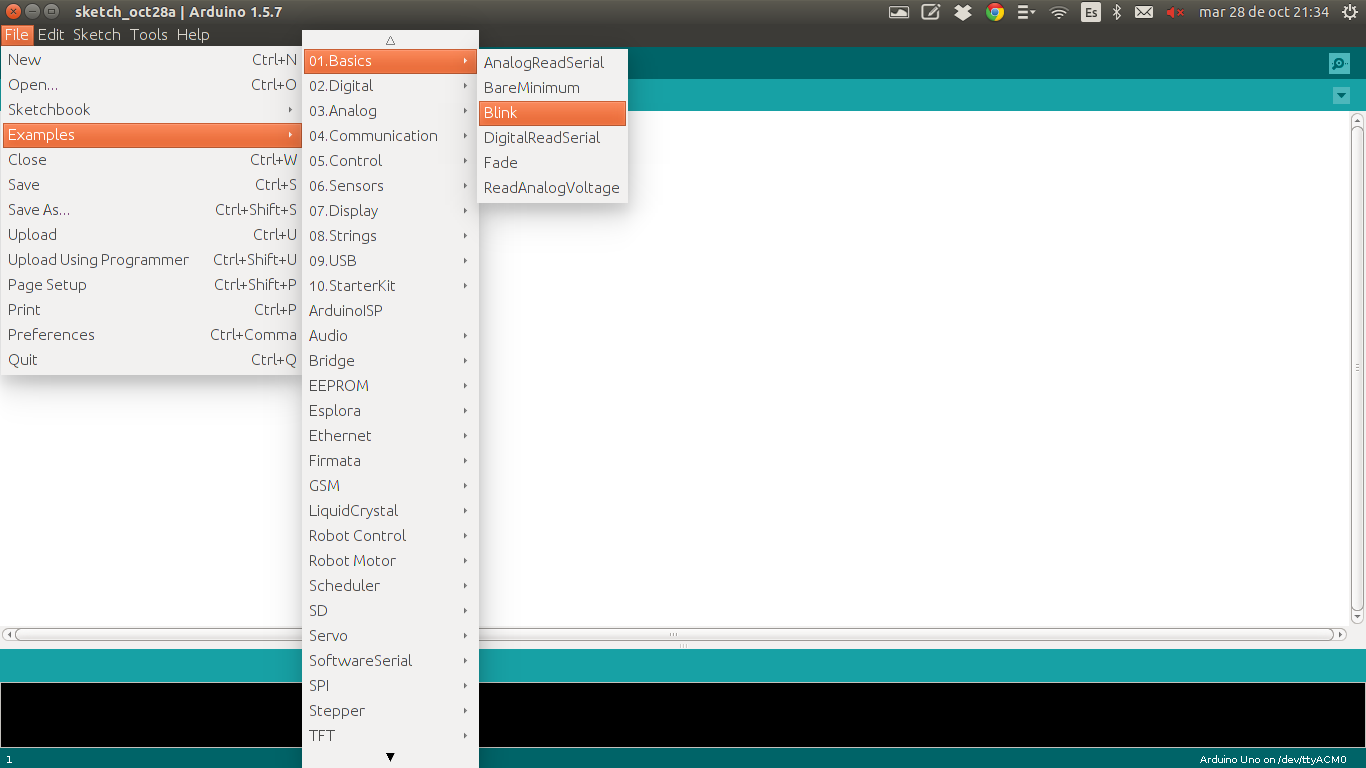
\includegraphics [width=0.8\textwidth]{open_blink.png}
\end{frame}

%______________________________________________________________________
\section{Arduino}

%......................................................................
\subsection{Intro}

%----------------------------------------------------------------------
\begin{frame}{SODAR}

FOTO DEL MONTAJE
  
\end{frame}

%----------------------------------------------------------------------
\begin{frame}{Arduino}

  \begin{figure}
    \centering
    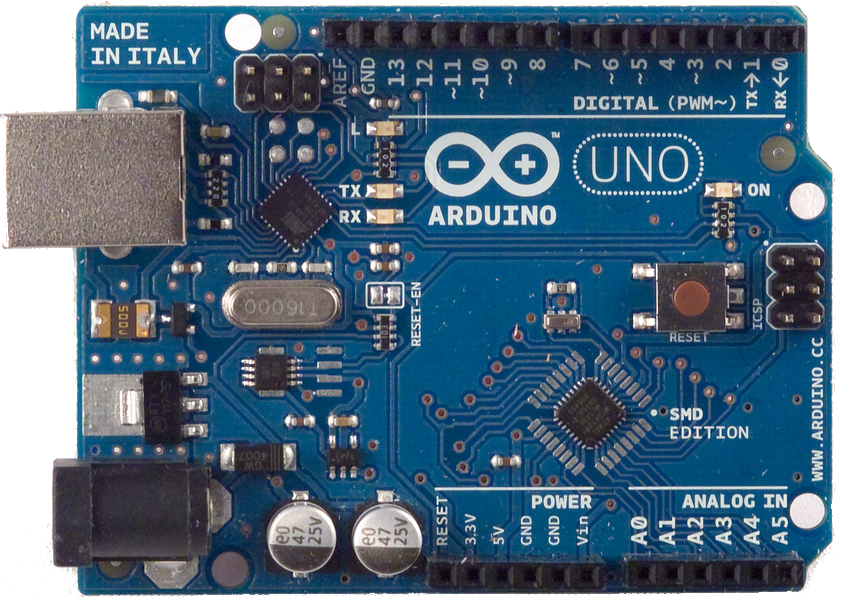
\includegraphics [width=0.7\textwidth]{ArduinoUnoSmd.jpg}
  \end{figure}
  \begin{columns}
    \column{.5\textwidth}
    \href{http://www.arduino.cc/}{Página Principal}
    \column{.5\textwidth}
    \href{http://blog.arduino.cc/wp-content/uploads/2013/11/ArduinoEvolution_make.jpg}{Foto Familia}
  \end{columns}
\end{frame}

%......................................................................
\subsection{Montaje}

%----------------------------------------------------------------------
\begin{frame}{Montaje I}
  Foto del soporte
\end{frame}

%----------------------------------------------------------------------
\begin{frame}{Montaje II}
  Esquema Fritzing
\end{frame}

%......................................................................
\subsection{Movimiento}

%----------------------------------------------------------------------
\begin{frame}[fragile]{Estructura de un programa Arduino}
\begin{lstlisting}
#include <Servo.h>     

#define SERVO_PWM_PIN 9

Servo myservo;         

/*----------------------------------------------------------------------
  setup
   Se ejecuta una sola vez al principio del programa. O cuando el arduino
   se resetea.
 ----------------------------------------------------------------------*/
void setup() {
  
}

/*----------------------------------------------------------------------
  loop
   Se ejecuta siempre, hasta el fin de los tiempos :-)
 ----------------------------------------------------------------------*/
void loop() {

}
\end{lstlisting}
\end{frame}

%----------------------------------------------------------------------
\begin{frame}{Servo}
  Foto del servo

  Fundido a Código de Invocación del servo
  
\end{frame}

%----------------------------------------------------------------------
\begin{frame}{Barridos}
  Foto de un radar (de verdad)
\end{frame}

%----------------------------------------------------------------------
\begin{frame}{Una solución}
  Nuestra solución
\end{frame}

%......................................................................
\subsection{Sensor}

%----------------------------------------------------------------------
\begin{frame}{Sensor ultrasonidos}
  Foto sensor

  Fundido a Caracteristicas técnicas
\end{frame}

%----------------------------------------------------------------------
\begin{frame}{Protocolo}
  Diagrama de señales
\end{frame}


\end{document}


